\documentclass{article}
\usepackage{authblk}
\usepackage{amsmath}
\usepackage{graphicx}
\usepackage{float}

\begin{document}
	\title{Comparison of the Numerical Solutions for the Radioactive Decay Equation Using Euler's Method and the Runge-Kutta Method.}
	\author{Daniel Reinhart \\ University of Central Florida \\ Orlando, FL, 32816}
	\date{}
	\affil{}
	
		\maketitle
	
\begin{abstract}
In this paper, we investigate the efficacy of two different numerical methods, Euler's method and the fourth order Runge-Kutta Method (RK4). The two methods are applied to the exactly solvable problem of radioactive decay, and compared to the analytical result.
\end{abstract}

\section{Radioactive Decay}
For a homogeneous sample of $N$ particles which have some probability to undergo radioactive decay, the change in particles $-dN$ in some time $dt$ should be proportional to the number of particles in the sample. In other words, the more particles we have the greater the chance of observing a decay is. We can therefore write the law governing this process as:

\begin{equation}
\frac{dN(t)}{dt}=-\alpha N(t)
\label{eqn1}
\end{equation}
This equation can be separated and integrated to yield:

\begin{equation}
N(t) = N_0 e^{-\alpha t},
\label{eqn2}
\end{equation}
where $N_0$ is the initial number of particles of the radioactive element. We can now see that $\alpha$ is just the reciprocal of the characteristic time:

\begin{equation}
N(t) = N_0 e^{-\frac{t}{\tau}}
\label{eqn3}
\end{equation}
For our analysis, we take the particles to be $^{238}Pu$ with characteristic time $\tau = 126.58 $ years.

\section{Euler's Mehtod}
Consider the first order differential equation with initial condition

\begin{equation}
\frac{dy}{dt}=f(y,t), \hspace{.2cm} y(t_0)=y_0
\label{eqn4}
\end{equation}
We wish to approximate a solution to this equation in general. So suppose we know the solution at some time $\xi$. Using the Taylor expansion of $y$ we find:

\begin{equation}
y(\xi+\Delta t) = y(\xi)+\frac{dy}{dt}_{t=\xi} \Delta t+O(\Delta t^2).
\label{eqn5}
\end{equation}
Upon using (\ref{eqn4}) we can write to first order in $\Delta t$

\begin{equation}
y(\xi+\Delta t) \approx y(\xi)+f(y,t)_{t=\xi}\Delta t
\label{eqn6}
\end{equation}
Using this method, we are continually accruing an error proportional to $\Delta t^2$ at each step of the approximation. If our final value of $t$ is $t_f$ then the number of approximations we make will be $N=\frac{t_f}{\Delta t}$, meaning the error at the end of our calculation will be proportional to $N \Delta t^2$, i.e. $O(\Delta t)$ (Giordano and Nakanishi \cite{GiordanoNakanishi}).

Returning to the problem of radioactive decay we obtain:

\begin{equation}
N(t+\Delta t) = N(t)(1-\frac{\Delta t}{\tau}).
\label{eqn7}
\end{equation}
This was implemented in Fortran, using step sizes of 6.329 years and 31.645 years for $^{238}Pu$ having a characteristic time $\tau = 126.58 $ . The data are plotted below:

\begin{figure}[H]
	\begin{center}
		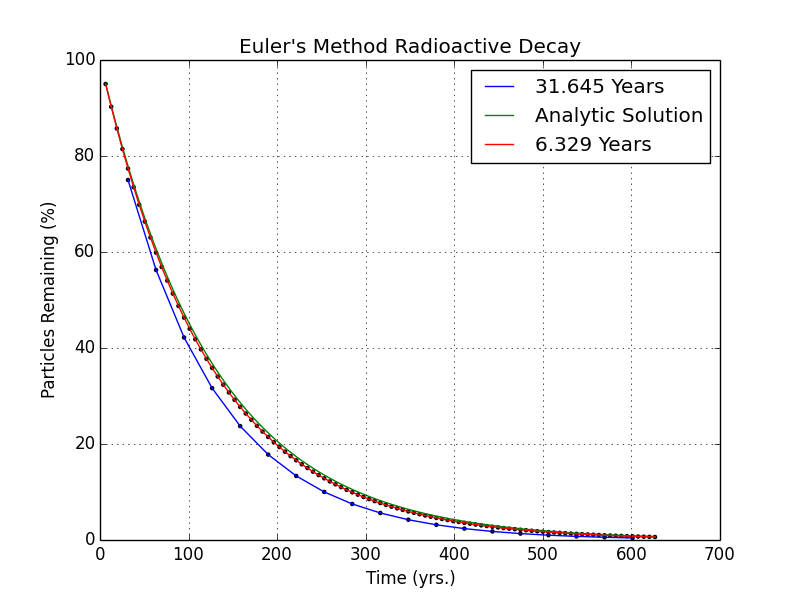
\includegraphics[scale=.5]{EulerPlots.png}
		\label{EulerPlots}
		\caption{Euler Method plots using time step sizes of 31.645 and 6.329 years.}
	\end{center}
\end{figure}
It is obvious that the method becomes a better approximation as the step size becomes smaller. The average percent error for the step size of 31.645 years was computed to be 29.93\%, while the average error for the step size of 6.329 years was .062\%.

There are many shortcomings of the Euler method. As was illustrated above, the method is not very accurate, especially compared to the RK4 method. The method also is not considered to be very stable (Press et al. \cite{Press}).

\section{Runge-Kutta}
The next method we explored was the fourth order Runge-Kutta method (RK4). The method is a little easier to understand for the second order, so we will walk through that derivation to build an understanding of the method. We again assume a first order system (\ref{eqn4}). We then observe:

\begin{equation}
y(t+\Delta t) \approx y(t)+ y'\Big(t+\frac{\Delta t}{2}\Big) \Delta t = y(t)+f\Big(y\Big(t+\frac{\Delta t}{2}\Big),t+\frac{\Delta t}{2}\Big)\Delta t
\label{eqn8}
\end{equation}
Taylor expanding $y\Big(t+\frac{\Delta t}{2}\Big)$, we arrive at the second order Runge-Kutta approximation:

\begin{equation}
y(t+\Delta t) \approx y(t)+ f\Big(y(t)+\frac{\Delta t}{2} f(y,t), t+\frac{\Delta t}{2}\Big)\Delta t.
\label{eqn9}
\end{equation}
This method is similar to the Euler method, except instead of sampling the slope at the beginning of the interval we sample at the midpoint.

The RK4 method, which is the best of the approximations so far, samples four points and uses a weighted average for the slope. The algorithmic approximation for the method is given below (Press et al. \cite{Press})

\begin{multline}
\\k_1= h f(y_n, t_n)\\
k_2 = h f\Big(y_n+\frac{k_1}{2},t_n+\frac{h}{2}\Big)\\
k_3 = h f\Big(y_n+\frac{k_2}{2},t_n+\frac{h}{2}\Big)\\
k_4 = h f(y_n+k_3,t_n+h)\\
y_{n+1} = y_n+\frac{k_1}{6}+\frac{k_2}{3}+\frac{k_3}{3}+\frac{k_4}{6}+O(h^5)\\
\label{eqn9}
\end{multline}

This algorithm was implemented for (\ref{eqn1}), and the results are plotted below:

\begin{figure}[H]
	\begin{center}
		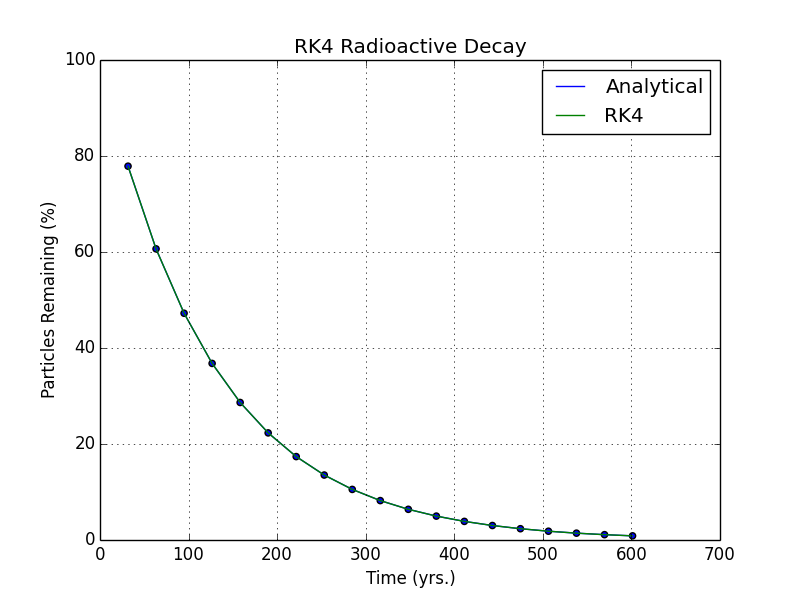
\includegraphics[scale=.5]{RK4.png}
		\label{RK4Plot}
		\caption{Plots of the RK4 method with the analytical solution. The time step used was 31.645 years.}
	\end{center}
\end{figure}
Just looking at the graph the fit appears to be a much better approximation than the Euler Method approximations, especially since we used the same step size as the worst of the Euler approximations. The average percent error for the RK4 method was .01\%. This is two orders of magnitude smaller than the Euler method using the same step size.

\section{Discussion}
Most problems in physics are not exactly solvable, and require numerical implementation in order to solve the equations involving the quantities of interest. For first order differential equations, a variety of methods exist regarding the approximation of solutions. We first studied the Euler Method, which is just the first order Taylor approximation for the solution. This method appeared to give okay results for small time steps. This is problematic since both accuracy and computing time scale at the same rate (Giordano and Nakanishi \cite{GiordanoNakanishi}). This will become problematic for complex problems. The next method we investigated was the Runge-Kutta fourth order method. This method employs the same underlying principle as the Euler method, except it uses a weighted average for the value of the derivative in the Taylor series. This method proved to be much better, with a faster rate of convergence than the Euler method. It appears as though the method that is desirable depends on how accurate you wish your approximation to be, and whether or not computation time matters with our algorithm.

\begin{thebibliography}{2}
	\bibitem{GiordanoNakanishi}
	N. J. Giordano and H. Nakanishi, \textit{Computational Physics}, Addison-Wesley, (2005).
	\bibitem{Press}
	W. H. Press, S. A. Teukolsky, W. T. Vetterling, B. P. Flannery, \textit{Numerical Recipes in C}, Cambridge University Press, (2002).
\end{thebibliography}

\end{document}

